\documentclass[10pt]{report}
\usepackage[utf8]{inputenc}
\usepackage[T1]{fontenc}
\usepackage{graphicx}
\usepackage[normalem]{ulem}
\usepackage{amsmath}
\usepackage{amssymb}
\usepackage{authblk}
\usepackage{minted}
\usepackage{titlepic}
\usepackage{booktabs}
% \title{$\vcenter{\hbox{\includegraphics[width=\linewidth]{images/ADM.jpeg}}}$ \\ Progetto Basi di Dati}
% \author{Buglione Giuseppe}
% \author{Calcagno Mario}
% \author{Calculli Francesco}
% \titlepic{\includegraphics[width=\linewidth]{images/F2.png}} % F2.png
% \affil{Dipartimento delle Tecnologie dell'Informazione, Università Federico II}
% \date{a.a. 2024/2025}
\begin{document}
% \maketitle
\begin{titlepage}
  \centering
  \includegraphics[width=0.75\linewidth]{images/ADM.jpeg}\par
  {\Large \textsc{\texttt{ASTRADM}}\par}
  {\Large\itshape Buglione Giuseppe\par}
  {\Large\itshape Calcagno Mario\par}
  {\Large\itshape Calculli Francesco\par}
  {\Large\itshape Dipartimento delle Tecnologie dell'Informazione, Università Federico II\par}
  \vfill
  \includegraphics[width=0.15\linewidth]{images/F2.png}
\end{titlepage}

\tableofcontents
\chapter{Introduzione}
% DONE: scrivere introduzione
% DONE: scegliere nome del programma
% DONE: scirvere specifica funzionale
% DONE: scrivere specifica sugli utenti e policy di sicurezza
\texttt{ASTRADM} nasce con l'intento di fornire un sistema informatico
per l'analisi e la gestione dei dati raccolti durante le missioni
d'esplorazione spaziali.  Il sistema permette da parte dei membri
dell'equipaggio una gestione completa delle informazioni provenienti
dai sensori e fornire un monitoraggio dettagliato delle operazioni in
corso.


% DONE: scrivere specifica informale
% DONE: risolvere il problema del da capo
\section{Specifica Informale} 
A.D.M. (Astra Data Management), un sistema informatico ,a supporto per i membri delle future missioni di esplorazioni lunari

\subsection{Obiettivi Principali:}
\begin{itemize}
\item  La gestione e analisi dei dati raccolti da sensori sparsi sulla superficie lunare 
\item  Gestione delle possibili anomalie riscontrabili e dei conseguenti interventi di riparazione.
\item  Gestori di robot autonomi per operazioni sul campo.
\item  Coordinazione in tempo reale della attivita dei membri della missione
\item  Monitoraggio delle operazioni in corso e dei relativi report.
\end{itemize}

%%% Local Variables:
%%% mode: LaTeX
%%% TeX-master: "Tesina"
%%% End:

% TODO: scrivere specifica sui dati
\section{Specifica sui dati}
Come visto già nella specifica informale, è necessario poter gestire i seguenti dati:
\subparagraph{Sensori}
\begin{description}
\item[ID] Il codice identificativo del singolo sensore
\item[Stato] Lo stato del sensore, così da poter gestire possibili
  errori di funzionamento
\item[Posizione] La posizione del sensore in coordinate classiche
  (latitudine, longitudine, altitudine)
\item[Ultimo Controllo] La data dell'ultimo controllo a cui è stato
  sottoposto il sensore, sempre per gestire anomalie
\item[Tipo] Il tipo di sensore
\item[Data di Installazione] La data di posizionamento e installazione
  del sensore
\end{description}
\subparagraph{Robot}
\begin{description}
\item[Codice] Il codice identificativo del singolo sensore
\item[Tipologia] Il tipo di robot utilizzato
\end{description}
\subparagraph{Missione}
\begin{description}
\item[Codice] Codice di identificazione univoca della missione
\item[Stato Attuale] Lo stato corrente della missione
\item[Obbiettivo] L'obbiettivo della missione
\item[Data Fine] La data in cui la missione è stata completata
\item[Data Inizio] La data di inizio della missione
\end{description}
\subparagraph{Report}
\begin{description}
\item[Stato] Lo stato del report
\end{description}
\subparagraph{Membro}
\begin{description}
\item[Codice] Codice di identificazione del membro d'equipaggio
\item[Nome e Cognome] I dati anagrafici della persona
\item[Ruolo] Il ruolo all'interno dell'equipaggio
\end{description}
\subparagraph{Anomalia}
\begin{description}
\item[Causa] La causa (certa o presunta) dell'anomalia
\item[Data e Ora] La date e l'ora del rilevamento dell'anomalia
\item[Livello] Il livello di gravità dell'anomalia
\end{description}
\subparagraph{Intervento}
\begin{description}
\item[Codice] Codice identificativo del singolo intervento
\item[Esito] L'esito dell'intervento
\item[Data] La data prefissata per l'esecuzione dell'intervento
\item[Descrizione] Il tipo dell'intervento
\end{description}
\subparagraph{Rilevazione}
\begin{description}
\item[Data e Ora] La data e ora del rilevamento
\item[Valore] Il valore rilevato
\end{description}

\section{Specifica delle funzionalità}
La piattaforma deve mettere a disponibilità le seguenti funzionalità:
\begin{itemize}
  \item Monitoraggio delle operazioni
  \item Gestione dei sensori sulla superficie lunare
  \item Supporto a diverse operazioni di analisi statistica
\end{itemize}
In particolare gli operatori devono essere in grado di:
\begin{itemize}
  \item Registrare o cancellare le missioni
  \item Registrare o cancellare le anomalie
  \item Inserire i report
\end{itemize}

%%% Local Variables:
%%% mode: LaTeX
%%% TeX-master: "Tesina"
%%% End:

\section{Specifica utenti e policy di sicurezza}
Creato lo schema della basi di dati:
\mint{sql}/CREATE SCHEMA ASTRADM;/
\par
Si è deciso di creare i seguenti utenti:
\begin{description}
\item[Database Administrator] DBA, con controllo completo della base di dati
  \begin{minted}{sql}
    CREATE USER astradm_dba IDENTIFIED BY astradm_dba;
    GRANT DBA TO astradm_dba;
  \end{minted}
\item[Admin] Amministratore di sistema, ha i permessi CREATE, DROP, INSERT,UPDATE, DELETE e SELECT, oltre alla
  possibilità di creare nuove stored procedures
  \begin{minted}{sql}
    CREATE ROLE admin;
    GRANT CONNECT TO admin;
    GRANT RESOURCE TO admin;
  \end{minted}
  %TODO: Rivedere creazione ruolo operator
\item[Operatore] Un operatore ha i permessi INSERT, UPDATE, DELETE, SELECT.
  \begin{minted}{sql}
    CREATE ROLE operator;
    GRANT CONNECT TO operator;
    GRANT SELECT ON ASTRADM.* TO operator;
    GRANT INSERT,UPDATE, DELETE ON ASTRADM.* TO operator
  \end{minted}
\end{description}

%%% Local Variables:
%%% mode: LaTeX
%%% TeX-master: "Tesina"
%%% End:


%%% Local Variables:
%%% mode: LaTeX
%%% TeX-master: "Tesina"
%%% End:

\chapter{Progettazione Concettuale}
In questa sezione si affronta la traduzione delle problematiche presentate in un
modello \textbf{Entity-Relationship}, abbreviato in ``E/R'', definendo le entità
e le relazioni che lo compongono.
% TODO: scrivere discussione dello schema ER portante
\paragraph{Schema E/R portante}
% TODO: definire schema ER portante

% TODO: Scrivere discussione dello schema ER finale
\section{Schema E/R finale}
Da una analisi più approfondia si vista la necessità di introdurre delle nuove entità:
\begin{description}
% TODO: aggiungere immagini entità
\item [Anomalia] con cui si va ad indicare un Sensore non funzionante.
\item [Intervento] per la riparazione di un Sensore non funzionante.
\item [Rilevazione] con cui si va indentificare i dati ralcolti dai sensori.
\end{description}
Caratterizate dalle seguenti relazioni:
\begin{description}
% TODO: Aggiungere immagini relazioni
\item [Analisi] che va a legare Rivelazioni e Sensore, con cui si va ad indicare i dati racolti dai vari sensori.
\item [Malfunzionamento] che va a legare Sensore ed Anomalia, tramite cui si individuano i sensori non funzionanti.
\item [Risoluzione] che va ad legare Anomalia ed Intervento, azine con cui si va ad riparere un sensore non funzionante.
\end{description}
Nel modello \ref{fig:er-portante} sono riporta le \textbf{cardinalita}specificando il numero minimo e il numero massimo che, le occorrenze, possono assumere in ciascuna associazione, rispetto alle entità. Le cardinalità delle relazioni sono le seguenti: 
\begin{description}
% TODO: Aggiungere immagini relazioni
\item[Partecipazione] di tipo \textbf{molti a molti (N,N)}; un membro
  dell'equipaggio può essere stato selezionato per la partecipazione
  di diverse missioni spaziali, mentre una missione richiede almeno un
  membro dell'equipaggio.
\item[Stesura] di tipo \textbf{molti a molti (N,N)}; un report può
  essere scritto da molteplici membri dell'equipaggio, mentre un
  membro dell'equipaggio può comporre diversi report.
\item[Report] di tipo \textbf{uno a molti (1,N)}; indica
  l'appartenenza di un report ad un'unica missione, quando invece una
  missione è composta da diversi report che informano dello stato
  della missione man mano.
\item[Risorsa\_1 e Risorsa\_2] entrambe di tipo \textbf{molti a molti
  (N,N)};in quanto una missione ha la possibilità di utilizzare
  molteplici sensori, quando un sensore viene ripiegato per una
  molteplicità di missioni. Analogalmente la relazione è identica per
  l'utilizzo dei robot nelle missioni.
\item[Malfunzionamento] di tipo \textbf{molti a molti (1,N)};
  in quanto quando si presenta un'anomalia, essa si riferisce ad un
  determinato sensore. Invece per i sensori vi è la possibilità di
  trovare diverse anomalie.
\item[Risoluzione] di tipo \textbf{uno a molti (1,N)} quando
  si presenta un'anomalia, un intervento può risolverla. Un intervento
  può essere applicato su diverse anomalie quando hanno la stessa
  causa;.
\item[Eseguito] di tipo \textbf{molti a molti (N,N)}; un
  membro dell'equipaggio può eseguire innumerevoli interventi. Un
  intervento ha la possibilità di essere eseguito, sia da nessun
  membro, che da molteplici membri.
\item[Analisi] di tipo \textbf{uno a molti (1,N)}; una
  rilevazione viene analizzata da un determinato sensore, il sensore
  invece effettua diverse rilevazioni.
\end{description}

\begin{figure}[ht]
  \centering
  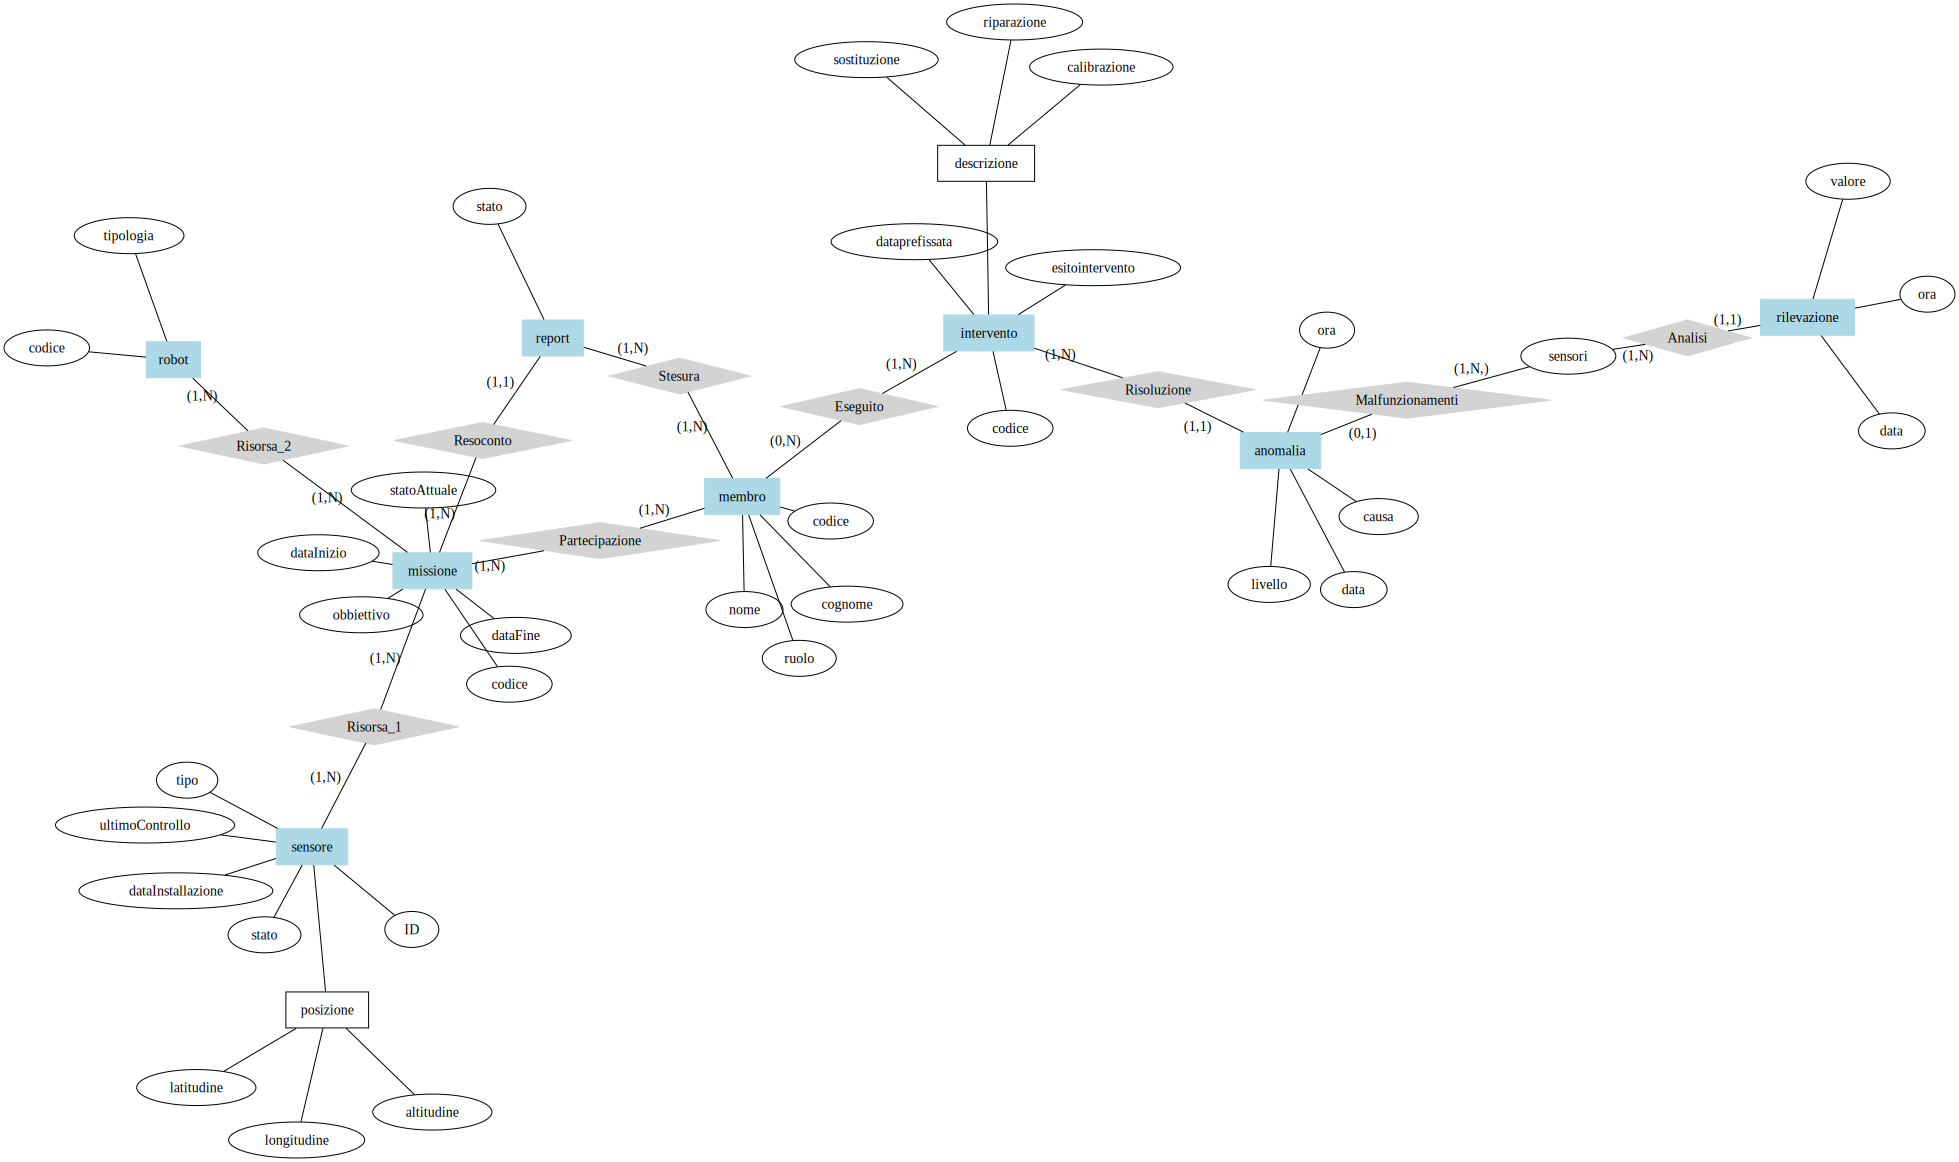
\includegraphics[width=\linewidth]{images/er.png}
  \caption{Modello E/R definitivo per \texttt{ASTRADM}}
  \label{fig:er}
\end{figure}


%%% Local Variables:
%%% mode: LaTeX
%%% TeX-master: "Tesina"
%%% End:


%%% Local Variables:
%%% mode: LaTeX
%%% TeX-master: "Tesina"
%%% End:

\chapter{Progettazione Logica}
Di qui si tratta della progettazione logica del database per
\texttt{ASTRADM}

\section{Trasformazione del modello E/R}
Riferendoci al modello raffigurato in \ref{fig:er} possiamo cominciare
a discutera della semplificazione e della specializzazione del
modello. Partendo dal modello \ref{fig:er} possiamo vedere come gli attributi:
\begin{description}
\item[descrizione] dell'entità \textbf{Intervento}
\item[posizione] dell'entità \textbf{Sensore}
\end{description}
siano composti. Di conseguenza è possibili trasformarli nel seguente modo:
\begin{center}
  descrizione $\rightarrow$ sostituzione,riparazione, calibrazione
\end{center}
e
\begin{center}
  posizione $\rightarrow$ latitudine, longitudine, altitudine
\end{center}

Di conseguenza il modello diventa
\begin{figure}[ht]
  \includegraphics[width=\linewidth]{images/er-finale.png}
  \caption{Modello ER finale per \texttt{ASTRADM}}
  \label{fig:er-finale}
\end{figure}
 	

%%% Local Variables:
%%% TeX-master: "Tesina.tex"
%%% End:

\section{Creazione Schema Relazionale}
In questa sezione ci occupiamo della creazione dello schema relazionale partendo dal
modello E/R in \ref{fig:er-finale}. Per la traduzione da modello E/R a schema relazionale
si seguono le seguenti regole:
\begin{enumarate}
\item Ciascuna \textit{entità} viene trasformata in una relazione,
  dove gli attributi dell'entità diventano gli attributi della
  relazione, con la chiave primaria dell'entità che diventa
  l'identificatore della relazione
\item Le relazioni vengono tradotte in base alla loro cardinalità:
  \begin{description}
  \item[uno a uno] si traducono aggiungendo alle relazioni che traducono le entità dal lato uno gli
    attributi delle associazioni e gli identificatori delle entità lato molti. Questi ultimi saranno soggetti
    ad un vincolo di integrità referenziale con il corrispondente attributo delle entità dal lato molti
  \item[uno a molti] si traducono aggiungendo alla relazione che traduce una delle due entità gli attributi
    dell’associazione, oltre che il suo identificatore che sarà soggetto sia ad un vincolo di unicità
    che di integrità referenziale con il corrispondente attributo dell’altra entità.
  \end{description}
\end{enumarate}

% TODO: Creare schema relazionale
Seguendo queste regole si ottiene il seguente schema:
\begin{itemize}
  % TODO: Completare SENSORE
\item \texttt{ANOMALIE}();
  % TODO: Completare SENSORE
\item \texttt{INTERVENTI}();
  % TODO: Completare SENSORE
\item \texttt{MEMBRI}();
  % TODO: Completare SENSORE
\item \texttt{MISSIONI}(\underline{codice},);
  % TODO: Completare SENSORE
\item \texttt{REPORT}();
  % TODO: Completare SENSORE
\item \texttt{RILEVAZIONI}();
  % TODO: Completare SENSORE
\item \texttt{ROBOT}();
  % TODO: Completare SENSORE
\item \texttt{SENSORI}();
\end{itemize}

%%% Local Variables:
%%% mode: LaTeX
%%% TeX-master: "Tesina"
%%% End:


%%% Local Variables:
%%% mode: LaTeX
%%% TeX-master: "Tesina"
%%% End:

\chapter{Progettazione Fisica}
<<<<<<< HEAD
=======
\section{Dimensionamento dei dati}
% TODO:Completare inserendo in numero di tuple
Per andare fare una stima sul volume che adranno ad occupare i vari dati in base allla loro tipologia, ci baseremo su:
\begin{itemize}
\item Tabelle/Schemi ottenute in fase di progettazione logica (sezione 3.2)
\item Il numero di missioni previste dall'agenzia spaziale
\end{itemize}
In questo caso ci baseremo per sul popolamento fatto nella sezione 4.4 per fare il dimensionamento.
\subsection{Anomalia}
\begin{tabular}{|c|c|c|}
  \hline
  \multicolumn{3}{|c|}{\textbf{ANOMALIA}}\\
  \hline
  Attributo & Tipo & Spazio(Byte) \\
  \hline
  data & DATE & 7 \\
  ora & VARCHAR(8)  & 8 \\
  causa & VARCHAR(30) & 30 \\
  livello & INTEGGER & 4 \\
  sensore & INTEGER & 4 \\
  \hline
\end{tabular}
\begin{equation}
  \begin{aligned}
    D{\text{\textsubscript{anomalia}}}&=(D{\text{\textsubscript{data}}} + D{\text{\textsubscript{ora}}} +D{\text{\textsubscript{causa}}} +D{\text{\textsubscript{livello}}} + D{\text{\textsubscript{sensore}}}) \cdot N{\text{\textsubscript{anomalie}}}=\\
    &=(7+8+30+4+4)\cdot 6 = 318\text{\textbf{B}}\\
  \end{aligned}
\end{equation}
\subsection{Interventi}
\begin{tabular}{ |c|c|c|}
  \hline
  \multicolumn{3}{|c|}{\textbf{INTERVENTI}} \\
  \hline
  Attributo & Tipo & Spazio(Byte) \\
  \hline
  codice & INTEGER & 4 \\
  esito & VARCHAR(20) & 20 \\
  calibrazione & VARCHAR(20) & 20 \\
  riparazione & VARCHAR(20) & 20 \\
  sostituzione & VARCHAR(20) & 20 \\
  dataPrefissata & DATE & 7 \\
  \hline
\end{tabular}
\begin{equation}
  \begin{aligned}
    D{\text{\textsubscript{interventi}}} &=(D{\text{\textsubscript{codice}}} + D{\text{\textsubscript{esito}}} +D{\text{\textsubscript{calibrazione}}} +D{\text{\textsubscript{riparazione}}} + D{\text{\textsubscript{sostituzione}}} + D{\text{\textsubscript{dataPrefissata}}}) \cdot  N{\text{\textsubscript{int}}} =\\
    &=(4+20+20+20+20+7)\cdot 5 = 455\textbf{B}
  \end{aligned}
\end{equation}
\subsection{Membri}
\begin{tabular}{ |c|c|c|}
  \hline
  \multicolumn{3}{|c|}{\textbf{MEMBRI}}\\
  \hline
  Attributo & Tipo & Spazio(Byte) \\
  \hline
  codice & INTEGER & 4 \\
  nome & VARCHAR(30) & 30 \\
  cognome & VARCHAR(30) & 30 \\
  ruolo & VARCHAR(30) & 30\\
  \hline
\end{tabular}
\begin{equation}
  \begin{aligned}
    D{\text{\textsubscript{membri}}} &=(D{\text{\textsubscript{codice}}} + D{\text{\textsubscript{nome}}} +D{\text{\textsubscript{cognome}}} +D{\text{\textsubscript{ruolo}}}) \cdot  N{\text{\textsubscript{membri}}} =\\
    &=(4+30+30+30) \cdot 5 = 470\textbf{B}
  \end{aligned}
\end{equation}
\subsection{Missioni}
\begin{tabular}{ |c|c|c|}
  \hline
  \multicolumn{3}{|c|}{\textbf{MISSIONI}}\\
  \hline
  Attributo & Tipo & Spazio(Byte) \\
  \hline
  codice & INTEGER & 4 \\
  dataFine & DATE & 7 \\
  obbiettivo & VARCHAR(100) & 100 \\
  dataInizio & DATE & 7 \\
  statoAttuale  & VARCHAR(30) & 30 \\
  resoconto & VARCHAR(30) & 30 \\
  \hline
\end{tabular}
\begin{equation}
  \begin{aligned}
    &D{\text{\textsubscript{missioni}}} =\\
    &=(D{\text{\textsubscript{codice}}}+D{\text{\textsubscript{dataFine}}}+D{\text{\textsubscript{obbietivo}}}+D{\text{\textsubscript{dataInizio}}}+D{\text{\textsubscript{statoA}}}+D{\text{\textsubscript{dataFine}}})\cdot N{\text{\textsubscript{miss}}}=\\
    &=(4+7+100+7+30+30)\cdot 5 = 890\textbf{B}
  \end{aligned}
\end{equation}
\subsection{Risorsa\textsubscript{1}}
\begin{tabular}{|c|c|c|}
  \hline
  \multicolumn{3}{|c|}{\textbf{RISORSA\textsubscript{1}}}\\
  \hline
  Attributo & Tipo & Spazio(Byte) \\
  \hline
  sensore & INTEGGER & 4 \\
  missione & INTEGER & 4 \\
  \hline
\end{tabular}
\begin{equation}
  \begin{aligned}
    D{\text{\textsubscript{risorsa1}}}&=(D{\text{\textsubscript{sensore}}} + D{\text{\textsubscript{missione}}}) \cdot N{\text{\textsubscript{risorse1}}}=\\
    &=(4+4)\cdot 5 = 40\text{\textbf{B}}\\
  \end{aligned}
\end{equation}
\subsection{Report}
\begin{tabular}{|c|c|c|}
  \hline
  \multicolumn{3}{|c|}{\textbf{REPORT}}\\
  \hline
  Attributo & Tipo & Spazio(Byte) \\
  \hline
  stato & VARCHAR(30) & 30 \\
  autore & INTEGER & 4\\
  \hline
\end{tabular}
\begin{equation}
  \begin{aligned}
    D{\text{\textsubscript{report}}} &=(D{\text{\textsubscript{stato}}}+D{\text{\textsubscript{autore}}})\cdot N{\text{\textsubscript{report}}}=\\
    &=(30+4)\cdot 5 = 170\textbf{B}
  \end{aligned}
\end{equation}
\subsection{Rilevazioni}
\begin{tabular}{|c|c|c|}
  \hline
  \multicolumn{3}{|c|}{\textbf{RILEVAZIONI}}\\
  \hline
  Attributo & Tipo & Spazio(Byte) \\
  \hline
  data & DATE & 7 \\
  ora & VARCHAR(8)  & 8\\
  valore & INTEGER & 4 \\
  sensore & INTEGER & 4 \\
  \hline
\end{tabular}
\begin{equation}
  \begin{aligned}
    D{\text{\textsubscript{rivelazione}}} &=\\
    &=(D{\text{\textsubscript{data}}}+D{\text{\textsubscript{ora}}}+D{\text{\textsubscript{valore}}}+D{\text{\textsubscript{sensore}}})\cdot N{\text{\textsubscript{rivelazione}}}=\\
    &=(7+8+4+4)\cdot 5 = 115\textbf{B}
  \end{aligned}
\end{equation}
\subsection{Robot}
\begin{tabular}{ |c|c|c|}
  \hline
  \multicolumn{3}{|c|}{\textbf{ROBOT}}\\
  \hline
  Attributo & Tipo & Spazio(Byte) \\
  \hline
  codice & INTEGER & 4\\
  tipologia & VARCHAR(30) & 30\\
  \hline
\end{tabular}
\begin{equation}
  \begin{aligned}
    D{\text{\textsubscript{robot}}} &=(D{\text{\textsubscript{codice}}}+D{\text{\textsubscript{tipologia}}})\cdot N{\text{\textsubscript{robot}}}=\\
    &=(4+30)\cdot 5 = 170\textbf{B}
  \end{aligned}
\end{equation}
\subsection{Sensori}
\begin{tabular}{ |c|c|c|}
  \hline
  \multicolumn{3}{|c|}{\textbf{SENSORI}}\\
  \hline
  Attributo & Tipo & Spazio(Byte) \\
  \hline
  ID & INTEGER & 4 \\
  stato & VARCHAR(30) & 30\\
  dataInstallazione & DATE & 7\\
  tipo & VARCHAR(30) & 30\\
  ultimoControllo & DATE & 7\\
  latitudine & DECIMAL(10,4) & 9\\
  altitudine & DECIMAL(10,4) & 9\\
  longitudine & DECIMAL(10,4) & 9\\
  \hline
\end{tabular}
\begin{equation}
  \begin{aligned}
    D_{\text{\textsubscript{sensore}}} &=\\
    &=(D{\text{\textsubscript{id}}}+D{\text{\textsubscript{stato}}}+D{\text{\textsubscript{dataInst}}}+D{\text{\textsubscript{ultCont}}}+D{\text{\textsubscript{lat}}}+D{\text{\textsubscript{alt}}}+D{\text{\textsubscript{long}}})\cdot N{\text{\textsubscript{sen}}}=\\
    &=(4+30+7+30+7+9+9+9)\cdot 5 = 525\textbf{B}
  \end{aligned}
\end{equation}
\subsection{Risorsa\textsubscript{2}}
\begin{tabular}{|c|c|c|}
  \hline
  \multicolumn{3}{|c|}{\textbf{RISORSA\textsubscript{2}}}\\
  \hline
  Attributo & Tipo & Spazio(Byte) \\
  \hline
  robot & INTEGGER & 4 \\
  missione & INTEGER & 4 \\
  \hline
\end{tabular}
\begin{equation}
  \begin{aligned}
    D{\text{\textsubscript{risorsa2}}}&=(D{\text{\textsubscript{robot}}} + D{\text{\textsubscript{missione}}}) \cdot N{\text{\textsubscript{risorse2}}}=\\
    &=(4+4)\cdot 6 = 48\text{\textbf{B}}\\
  \end{aligned}
\end{equation}
\subsection{Gestione dello spazio e dell'affidabilità}
Dalle stime fatte precedentemente possiamo stimare un volume di informazioni pari:
\begin{equation}
  D_{\text{tot}}=(318+455+470+890+40+170+115+170+525+48)= 3201\text{\textbf{B}}\\
\end{equation}

%%% Local Variables:
%%% mode: LaTeX
%%% TeX-master: "Tesina"
%%% End:

\section{Creazione del database}
%DONE: Da completare
Delineato il modello logico, tramite i comandi DDL possiamo inserire all'interno del data base gli schemi di relazioni associate alle tabelle.
\begin{description}

\subsection{Sensori}
\begin{minted}{sql}
CREATE SEQUENCE sensori_id_seq START WITH 1;
CREATE TABLE SENSORI (
    ID INTEGER DEFAULT sensori_id_seq.nextval NOT NULL,
    STATO VARCHAR(30) NOT NULL,
    DATAINSTALLAZIONE DATE NOT NULL,
    TIPO VARCHAR(30) NOT NULL,
    UTLIMOCONTROLLO DATE,
    LATITUDINE DECIMAL(10,4) NOT NULL,
    LONGITUDINE DECIMAL(10,4) NOT NULL,
    ALTITUDINE DECIMAL(10,4) NOT NULL,
    
    CONSTRAINT PK_ID PRIMARY KEY(ID)
    
    );
\end{minted}

\subsection{Anomalie}
\begin{minted}{sql}
CREATE TABLE ANOMALIE(
    DATA DATE NOT NULL,
    ORA DATE NOT NULL,
    CAUSA VARCHAR(30) NOT NULL,
    LIVELLO INTEGER NOT NULL,
    SENSORE INTEGER NOT NULL,
    CONSTRAINT PK_ANOMALIE PRIMARY KEY (DATA,ORA),
    CONSTRAINT FK_ANOMALIE_SENSORI FOREIGN KEY (SENSORE) REFERENCES SENSORI (ID) ON DELETE CASCADE
    );
\end{minted}

\subsection{Interventi}
\begin{minted}[breaklines]{sql}
CREATE SEQUENCE interventi_codice_seq START WITH 1;
CREATE TABLE INTERVENTI(
    CODICE INTEGER DEFAULT interventi_codice_seq.nextval NOT NULL,
    ESITO VARCHAR(20) NOT NULL,
    CALIBRAZIONE VARCHAR(20) NOT NULL,
    RIPARAZIONE VARCHAR(20) NOT NULL,
    SOSTITUZIONE VARCHAR(20) NOT NULL,
    DATAPREFISSATA DATE NOT NULL,
    
    CONSTRAINT PK_INTERVENTI PRIMARY KEY(CODICE)
    );
\end{minted}

\subsection{Membri}
\begin{minted}[breaklines]{sql}
CREATE SEQUENCE membri_codice_seq START WITH 1;
CREATE TABLE MEMBRI(
    CODICE INTEGER DEFAULT membri_codice_seq.nextval NOT NULL,
    NOME VARCHAR(20) NOT NULL,
    COGNOME VARCHAR(20) NOT NULL,
    RUOLO VARCHAR(20) NOT NULL,
    
    CONSTRAINT PK_MEMBRI PRIMARY KEY(CODICE)
    );
\end{minted}

\subsection{Report}
\begin{minted}[breaklines]{sql}
CREATE TABLE REPORT(
    STATO VARCHAR(30) NOT NULL,
    AUTORE INTEGER NOT NULL,
    
    CONSTRAINT PK_REPORT PRIMARY KEY(STATO),
    CONSTRAINT FK_REPORT_MEMBRI FOREIGN KEY(AUTORE) REFERENCES MEMBRI(CODICE) ON DELETE CASCADE
    );
\end{minted}

\subsection{Missioni}
\begin{minted}[breaklines]{sql}
CREATE SEQUENCE missioni_codice_seq START WITH 1;
CREATE TABLE MISSIONI(
    CODICE INTEGER DEFAULT missioni_codice_seq.nextval NOT NULL,
    DATAFINE DATE NOT NULL,
    OBBIETTIVO VARCHAR(100) NOT NULL,
    DATAINIZIO DATE NOT NULL,
    STATOATTUALE VARCHAR(30) NOT NULL,
    RESOCONTO VARCHAR(30) NOT NULL,
    
    CONSTRAINT PK_MISSIONI PRIMARY KEY (CODICE),
    CONSTRAINT FK_MISSIONI_REPORT FOREIGN KEY (RESOCONTO) REFERENCES REPORT(STATO) ON DELETE CASCADE
);
\end{minted}

\subsection{Rilevazioni}
\begin{minted}[breaklines]{sql}
CREATE TABLE RILEVAZIONI(
    DATA DATE NOT NULL,
    ORA DATE NOT NULL, 
    VALORE INTEGER NOT NULL,
    SENSORE INTEGER NOT NULL,
    
    CONSTRAINT PK_RILEVAZIONI PRIMARY KEY(DATA,ORA),
    CONSTRAINT FK_RILEVAZIONI_SENSORI FOREIGN KEY(SENSORE) REFERENCES SENSORI (ID) ON DELETE CASCADE
)
\end{minted}

\subsection{Robot}
\begin{minted}[breaklines]{sql}
CREATE SEQUENCE robot_codice_seq START WITH 1;
CREATE TABLE ROBOT(
    CODICE INTEGER DEFAULT robot_codice_seq.nextval NOT NULL,
    TIPOLOGIA VARCHAR(30),
    
    CONSTRAINT PK_ROBOT PRIMARY KEY(CODICE)
    );
\end{minted}

\subsection{Risorsa\textsubscript{1}}
\begin{minted}[breaklines]{sql}
CREATE TABLE RISORSA_1(
    ROBOT INTEGER NOT NULL,
    MISSIONE INTEGER NOT NULL,
    CONSTRAINT PK_RISORSA_1 PRIMARY KEY(ROBOT,MISSIONE),
    CONSTRAINT FK_RISORSA1_ROBOT FOREIGN KEY(ROBOT) REFERENCES ROBOT(CODICE) ON DELETE CASCADE, 
    CONSTRAINT FK_RISORSA1_MISSIONE FOREIGN KEY(MISSIONE) REFERENCES MISSIONI(CODICE) ON DELETE CASCADE
    );
\end{minted}

\subsection{Risorsa\textsubscript{2}}
\begin{minted}[breaklines]{sql}
CREATE TABLE RISORSA_2(
    SENSORE INTEGER NOT NULL,
    MISSIONE INTEGER NOT NULL,
    
    CONSTRAINT PK_RISORSA_2 PRIMARY KEY (SENSORE,MISSIONE),
    CONSTRAINT FK_RISORSA2_SENSORE FOREIGN KEY(SENSORE) REFERENCES SENSORI(ID) ON DELETE CASCADE,
    CONSTRAINT FK_RISORSA2_MISSIONE FOREIGN KEY(MISSIONE) REFERENCES MISSIONI(CODICE) ON DELETE CASCADE
    
    );
\end{minted}
\end{description}


%%% Local Variables:
%%% mode: LaTeX
%%% TeX-master: "Tesina"
%%% End:

>>>>>>> 81b2a95e7ccb38f3d731b3ef867daf574a26ff44
%TODO: fare Dimensionamento dei dati
\section{Dimensionamento dei dati}
% TODO:Completare inserendo in numero di tuple
Per andare fare una stima sul volume che adranno ad occupare i vari dati in base allla loro tipologia, ci baseremo su:
\begin{itemize}
\item Tabelle/Schemi ottenute in fase di progettazione logica (sezione 3.2)
\item Il numero di missioni previste dall'agenzia spaziale
\end{itemize}
In questo caso ci baseremo per sul popolamento fatto nella sezione 4.4 per fare il dimensionamento.
\subsection{Anomalia}
\begin{tabular}{|c|c|c|}
  \hline
  \multicolumn{3}{|c|}{\textbf{ANOMALIA}}\\
  \hline
  Attributo & Tipo & Spazio(Byte) \\
  \hline
  data & DATE & 7 \\
  ora & VARCHAR(8)  & 8 \\
  causa & VARCHAR(30) & 30 \\
  livello & INTEGGER & 4 \\
  sensore & INTEGER & 4 \\
  \hline
\end{tabular}
\begin{equation}
  \begin{aligned}
    D{\text{\textsubscript{anomalia}}}&=(D{\text{\textsubscript{data}}} + D{\text{\textsubscript{ora}}} +D{\text{\textsubscript{causa}}} +D{\text{\textsubscript{livello}}} + D{\text{\textsubscript{sensore}}}) \cdot N{\text{\textsubscript{anomalie}}}=\\
    &=(7+8+30+4+4)\cdot 6 = 318\text{\textbf{B}}\\
  \end{aligned}
\end{equation}
\subsection{Interventi}
\begin{tabular}{ |c|c|c|}
  \hline
  \multicolumn{3}{|c|}{\textbf{INTERVENTI}} \\
  \hline
  Attributo & Tipo & Spazio(Byte) \\
  \hline
  codice & INTEGER & 4 \\
  esito & VARCHAR(20) & 20 \\
  calibrazione & VARCHAR(20) & 20 \\
  riparazione & VARCHAR(20) & 20 \\
  sostituzione & VARCHAR(20) & 20 \\
  dataPrefissata & DATE & 7 \\
  \hline
\end{tabular}
\begin{equation}
  \begin{aligned}
    D{\text{\textsubscript{interventi}}} &=(D{\text{\textsubscript{codice}}} + D{\text{\textsubscript{esito}}} +D{\text{\textsubscript{calibrazione}}} +D{\text{\textsubscript{riparazione}}} + D{\text{\textsubscript{sostituzione}}} + D{\text{\textsubscript{dataPrefissata}}}) \cdot  N{\text{\textsubscript{int}}} =\\
    &=(4+20+20+20+20+7)\cdot 5 = 455\textbf{B}
  \end{aligned}
\end{equation}
\subsection{Membri}
\begin{tabular}{ |c|c|c|}
  \hline
  \multicolumn{3}{|c|}{\textbf{MEMBRI}}\\
  \hline
  Attributo & Tipo & Spazio(Byte) \\
  \hline
  codice & INTEGER & 4 \\
  nome & VARCHAR(30) & 30 \\
  cognome & VARCHAR(30) & 30 \\
  ruolo & VARCHAR(30) & 30\\
  \hline
\end{tabular}
\begin{equation}
  \begin{aligned}
    D{\text{\textsubscript{membri}}} &=(D{\text{\textsubscript{codice}}} + D{\text{\textsubscript{nome}}} +D{\text{\textsubscript{cognome}}} +D{\text{\textsubscript{ruolo}}}) \cdot  N{\text{\textsubscript{membri}}} =\\
    &=(4+30+30+30) \cdot 5 = 470\textbf{B}
  \end{aligned}
\end{equation}
\subsection{Missioni}
\begin{tabular}{ |c|c|c|}
  \hline
  \multicolumn{3}{|c|}{\textbf{MISSIONI}}\\
  \hline
  Attributo & Tipo & Spazio(Byte) \\
  \hline
  codice & INTEGER & 4 \\
  dataFine & DATE & 7 \\
  obbiettivo & VARCHAR(100) & 100 \\
  dataInizio & DATE & 7 \\
  statoAttuale  & VARCHAR(30) & 30 \\
  resoconto & VARCHAR(30) & 30 \\
  \hline
\end{tabular}
\begin{equation}
  \begin{aligned}
    &D{\text{\textsubscript{missioni}}} =\\
    &=(D{\text{\textsubscript{codice}}}+D{\text{\textsubscript{dataFine}}}+D{\text{\textsubscript{obbietivo}}}+D{\text{\textsubscript{dataInizio}}}+D{\text{\textsubscript{statoA}}}+D{\text{\textsubscript{dataFine}}})\cdot N{\text{\textsubscript{miss}}}=\\
    &=(4+7+100+7+30+30)\cdot 5 = 890\textbf{B}
  \end{aligned}
\end{equation}
\subsection{Risorsa\textsubscript{1}}
\begin{tabular}{|c|c|c|}
  \hline
  \multicolumn{3}{|c|}{\textbf{RISORSA\textsubscript{1}}}\\
  \hline
  Attributo & Tipo & Spazio(Byte) \\
  \hline
  sensore & INTEGGER & 4 \\
  missione & INTEGER & 4 \\
  \hline
\end{tabular}
\begin{equation}
  \begin{aligned}
    D{\text{\textsubscript{risorsa1}}}&=(D{\text{\textsubscript{sensore}}} + D{\text{\textsubscript{missione}}}) \cdot N{\text{\textsubscript{risorse1}}}=\\
    &=(4+4)\cdot 5 = 40\text{\textbf{B}}\\
  \end{aligned}
\end{equation}
\subsection{Report}
\begin{tabular}{|c|c|c|}
  \hline
  \multicolumn{3}{|c|}{\textbf{REPORT}}\\
  \hline
  Attributo & Tipo & Spazio(Byte) \\
  \hline
  stato & VARCHAR(30) & 30 \\
  autore & INTEGER & 4\\
  \hline
\end{tabular}
\begin{equation}
  \begin{aligned}
    D{\text{\textsubscript{report}}} &=(D{\text{\textsubscript{stato}}}+D{\text{\textsubscript{autore}}})\cdot N{\text{\textsubscript{report}}}=\\
    &=(30+4)\cdot 5 = 170\textbf{B}
  \end{aligned}
\end{equation}
\subsection{Rilevazioni}
\begin{tabular}{|c|c|c|}
  \hline
  \multicolumn{3}{|c|}{\textbf{RILEVAZIONI}}\\
  \hline
  Attributo & Tipo & Spazio(Byte) \\
  \hline
  data & DATE & 7 \\
  ora & VARCHAR(8)  & 8\\
  valore & INTEGER & 4 \\
  sensore & INTEGER & 4 \\
  \hline
\end{tabular}
\begin{equation}
  \begin{aligned}
    D{\text{\textsubscript{rivelazione}}} &=\\
    &=(D{\text{\textsubscript{data}}}+D{\text{\textsubscript{ora}}}+D{\text{\textsubscript{valore}}}+D{\text{\textsubscript{sensore}}})\cdot N{\text{\textsubscript{rivelazione}}}=\\
    &=(7+8+4+4)\cdot 5 = 115\textbf{B}
  \end{aligned}
\end{equation}
\subsection{Robot}
\begin{tabular}{ |c|c|c|}
  \hline
  \multicolumn{3}{|c|}{\textbf{ROBOT}}\\
  \hline
  Attributo & Tipo & Spazio(Byte) \\
  \hline
  codice & INTEGER & 4\\
  tipologia & VARCHAR(30) & 30\\
  \hline
\end{tabular}
\begin{equation}
  \begin{aligned}
    D{\text{\textsubscript{robot}}} &=(D{\text{\textsubscript{codice}}}+D{\text{\textsubscript{tipologia}}})\cdot N{\text{\textsubscript{robot}}}=\\
    &=(4+30)\cdot 5 = 170\textbf{B}
  \end{aligned}
\end{equation}
\subsection{Sensori}
\begin{tabular}{ |c|c|c|}
  \hline
  \multicolumn{3}{|c|}{\textbf{SENSORI}}\\
  \hline
  Attributo & Tipo & Spazio(Byte) \\
  \hline
  ID & INTEGER & 4 \\
  stato & VARCHAR(30) & 30\\
  dataInstallazione & DATE & 7\\
  tipo & VARCHAR(30) & 30\\
  ultimoControllo & DATE & 7\\
  latitudine & DECIMAL(10,4) & 9\\
  altitudine & DECIMAL(10,4) & 9\\
  longitudine & DECIMAL(10,4) & 9\\
  \hline
\end{tabular}
\begin{equation}
  \begin{aligned}
    D_{\text{\textsubscript{sensore}}} &=\\
    &=(D{\text{\textsubscript{id}}}+D{\text{\textsubscript{stato}}}+D{\text{\textsubscript{dataInst}}}+D{\text{\textsubscript{ultCont}}}+D{\text{\textsubscript{lat}}}+D{\text{\textsubscript{alt}}}+D{\text{\textsubscript{long}}})\cdot N{\text{\textsubscript{sen}}}=\\
    &=(4+30+7+30+7+9+9+9)\cdot 5 = 525\textbf{B}
  \end{aligned}
\end{equation}
\subsection{Risorsa\textsubscript{2}}
\begin{tabular}{|c|c|c|}
  \hline
  \multicolumn{3}{|c|}{\textbf{RISORSA\textsubscript{2}}}\\
  \hline
  Attributo & Tipo & Spazio(Byte) \\
  \hline
  robot & INTEGGER & 4 \\
  missione & INTEGER & 4 \\
  \hline
\end{tabular}
\begin{equation}
  \begin{aligned}
    D{\text{\textsubscript{risorsa2}}}&=(D{\text{\textsubscript{robot}}} + D{\text{\textsubscript{missione}}}) \cdot N{\text{\textsubscript{risorse2}}}=\\
    &=(4+4)\cdot 6 = 48\text{\textbf{B}}\\
  \end{aligned}
\end{equation}
\subsection{Gestione dello spazio e dell'affidabilità}
Dalle stime fatte precedentemente possiamo stimare un volume di informazioni pari:
\begin{equation}
  D_{\text{tot}}=(318+455+470+890+40+170+115+170+525+48)= 3201\text{\textbf{B}}\\
\end{equation}

%%% Local Variables:
%%% mode: LaTeX
%%% TeX-master: "Tesina"
%%% End:

%TODO: fare Creazione del database
\section{Creazione del database}
%DONE: Da completare
Delineato il modello logico, tramite i comandi DDL possiamo inserire all'interno del data base gli schemi di relazioni associate alle tabelle.
\begin{description}

\subsection{Sensori}
\begin{minted}{sql}
CREATE SEQUENCE sensori_id_seq START WITH 1;
CREATE TABLE SENSORI (
    ID INTEGER DEFAULT sensori_id_seq.nextval NOT NULL,
    STATO VARCHAR(30) NOT NULL,
    DATAINSTALLAZIONE DATE NOT NULL,
    TIPO VARCHAR(30) NOT NULL,
    UTLIMOCONTROLLO DATE,
    LATITUDINE DECIMAL(10,4) NOT NULL,
    LONGITUDINE DECIMAL(10,4) NOT NULL,
    ALTITUDINE DECIMAL(10,4) NOT NULL,
    
    CONSTRAINT PK_ID PRIMARY KEY(ID)
    
    );
\end{minted}

\subsection{Anomalie}
\begin{minted}{sql}
CREATE TABLE ANOMALIE(
    DATA DATE NOT NULL,
    ORA DATE NOT NULL,
    CAUSA VARCHAR(30) NOT NULL,
    LIVELLO INTEGER NOT NULL,
    SENSORE INTEGER NOT NULL,
    CONSTRAINT PK_ANOMALIE PRIMARY KEY (DATA,ORA),
    CONSTRAINT FK_ANOMALIE_SENSORI FOREIGN KEY (SENSORE) REFERENCES SENSORI (ID) ON DELETE CASCADE
    );
\end{minted}

\subsection{Interventi}
\begin{minted}[breaklines]{sql}
CREATE SEQUENCE interventi_codice_seq START WITH 1;
CREATE TABLE INTERVENTI(
    CODICE INTEGER DEFAULT interventi_codice_seq.nextval NOT NULL,
    ESITO VARCHAR(20) NOT NULL,
    CALIBRAZIONE VARCHAR(20) NOT NULL,
    RIPARAZIONE VARCHAR(20) NOT NULL,
    SOSTITUZIONE VARCHAR(20) NOT NULL,
    DATAPREFISSATA DATE NOT NULL,
    
    CONSTRAINT PK_INTERVENTI PRIMARY KEY(CODICE)
    );
\end{minted}

\subsection{Membri}
\begin{minted}[breaklines]{sql}
CREATE SEQUENCE membri_codice_seq START WITH 1;
CREATE TABLE MEMBRI(
    CODICE INTEGER DEFAULT membri_codice_seq.nextval NOT NULL,
    NOME VARCHAR(20) NOT NULL,
    COGNOME VARCHAR(20) NOT NULL,
    RUOLO VARCHAR(20) NOT NULL,
    
    CONSTRAINT PK_MEMBRI PRIMARY KEY(CODICE)
    );
\end{minted}

\subsection{Report}
\begin{minted}[breaklines]{sql}
CREATE TABLE REPORT(
    STATO VARCHAR(30) NOT NULL,
    AUTORE INTEGER NOT NULL,
    
    CONSTRAINT PK_REPORT PRIMARY KEY(STATO),
    CONSTRAINT FK_REPORT_MEMBRI FOREIGN KEY(AUTORE) REFERENCES MEMBRI(CODICE) ON DELETE CASCADE
    );
\end{minted}

\subsection{Missioni}
\begin{minted}[breaklines]{sql}
CREATE SEQUENCE missioni_codice_seq START WITH 1;
CREATE TABLE MISSIONI(
    CODICE INTEGER DEFAULT missioni_codice_seq.nextval NOT NULL,
    DATAFINE DATE NOT NULL,
    OBBIETTIVO VARCHAR(100) NOT NULL,
    DATAINIZIO DATE NOT NULL,
    STATOATTUALE VARCHAR(30) NOT NULL,
    RESOCONTO VARCHAR(30) NOT NULL,
    
    CONSTRAINT PK_MISSIONI PRIMARY KEY (CODICE),
    CONSTRAINT FK_MISSIONI_REPORT FOREIGN KEY (RESOCONTO) REFERENCES REPORT(STATO) ON DELETE CASCADE
);
\end{minted}

\subsection{Rilevazioni}
\begin{minted}[breaklines]{sql}
CREATE TABLE RILEVAZIONI(
    DATA DATE NOT NULL,
    ORA DATE NOT NULL, 
    VALORE INTEGER NOT NULL,
    SENSORE INTEGER NOT NULL,
    
    CONSTRAINT PK_RILEVAZIONI PRIMARY KEY(DATA,ORA),
    CONSTRAINT FK_RILEVAZIONI_SENSORI FOREIGN KEY(SENSORE) REFERENCES SENSORI (ID) ON DELETE CASCADE
)
\end{minted}

\subsection{Robot}
\begin{minted}[breaklines]{sql}
CREATE SEQUENCE robot_codice_seq START WITH 1;
CREATE TABLE ROBOT(
    CODICE INTEGER DEFAULT robot_codice_seq.nextval NOT NULL,
    TIPOLOGIA VARCHAR(30),
    
    CONSTRAINT PK_ROBOT PRIMARY KEY(CODICE)
    );
\end{minted}

\subsection{Risorsa\textsubscript{1}}
\begin{minted}[breaklines]{sql}
CREATE TABLE RISORSA_1(
    ROBOT INTEGER NOT NULL,
    MISSIONE INTEGER NOT NULL,
    CONSTRAINT PK_RISORSA_1 PRIMARY KEY(ROBOT,MISSIONE),
    CONSTRAINT FK_RISORSA1_ROBOT FOREIGN KEY(ROBOT) REFERENCES ROBOT(CODICE) ON DELETE CASCADE, 
    CONSTRAINT FK_RISORSA1_MISSIONE FOREIGN KEY(MISSIONE) REFERENCES MISSIONI(CODICE) ON DELETE CASCADE
    );
\end{minted}

\subsection{Risorsa\textsubscript{2}}
\begin{minted}[breaklines]{sql}
CREATE TABLE RISORSA_2(
    SENSORE INTEGER NOT NULL,
    MISSIONE INTEGER NOT NULL,
    
    CONSTRAINT PK_RISORSA_2 PRIMARY KEY (SENSORE,MISSIONE),
    CONSTRAINT FK_RISORSA2_SENSORE FOREIGN KEY(SENSORE) REFERENCES SENSORI(ID) ON DELETE CASCADE,
    CONSTRAINT FK_RISORSA2_MISSIONE FOREIGN KEY(MISSIONE) REFERENCES MISSIONI(CODICE) ON DELETE CASCADE
    
    );
\end{minted}
\end{description}


%%% Local Variables:
%%% mode: LaTeX
%%% TeX-master: "Tesina"
%%% End:

%TODO: fare Gestione degli indici
<<<<<<< HEAD
\section{Gestione degli indici}
\mint{sql}/ /
%TODO: Da completare
Gli indici sono struttura dati ordinata impiegata nel DBMS per la localizzazione di un specifico record andando ad velocizzare le operazioni di ricerca, sono 
caratterizati da una data entry (record memorizato in un file indice) che può essere costituito:
\begin{itemize}
\item Intero record di dati
\item Coppia costituita da una \texttt{chiave} e \texttt{rid}
\item Coppia costituita da una \texttt{chiave} e \texttt{lista di rid}
\end{itemize}
Dove in \texttt{DBMS Oracle} va creare in maniera automati indici di tipo \texttt{B+Tree} per ogni chiave primaria di tutte le tabelle.
\begin{description}
\begin{minted}{sql}
 CREATE INDEX INTERVENTI_CODICE ON INTERVENTI (codice);
 CREATE INDEX REPORT_STATO ON REPORT (stato);
 CREATE INDEX ANOMALIE_DATA_ORA ON ANOMALIE (data, ora);
 CREATE INDEX RIVELAZIONI_DATA_ORA ON RIVELAZIONI (data, ora);
 CREATE INDEX MISSIONI_CODICE ON MISSIONI (codice);
\end{minted}
\end{description}

%%% Local Variables:
%%% mode: LaTeX
%%% TeX-master: "Tesina"
%%% End:
%TODO: fare Popolamento della base di dati
\section{Popolamento della base di dati}
%TODO: In caso di cambiamentoi nel popolamento ricardare di aggiornare il dimensionamento
In tale sezioni ci occuperemo del popolamento della base dati con l'ausilio di Chatgip per la creazione di dati fittizi con il fini di testare la nostra base dati. In otteniamo:
\begin{itemize}
\item 5 Sensori
\item 6 Anomalie
\item 5 Interventi
\item 5 Membri
\item 5 Report
\item 5 Missioni
\item 5 Rilevazioni
\item 5 Robot
\item 5 Risorsa\_1
\item 6 Risorsa\_2
\end{itemize}
\subsection{\texttt{Sensori}}
\begin{minted}[breaklines]{sql}
INSERT INTO SENSORI (STATO, DATAINSTALLAZIONE, TIPO, ULTIMOCONTROLLO, LATITUDINE, LONGITUDINE, ALTITUDINE) VALUES
('Attivo', TO_DATE('2023-01-15', 'YYYY-MM-DD'), 'Temperatura', TO_DATE('2024-02-01', 'YYYY-MM-DD'), 45.1234, 12.5678, 100.5),
('Guasto', TO_DATE('2022-06-20', 'YYYY-MM-DD'), 'Pressione', TO_DATE('2024-01-10', 'YYYY-MM-DD'), 44.8765, 13.6789, 200.3),
('Attivo', TO_DATE('2023-03-10', 'YYYY-MM-DD'), 'Umidità', TO_DATE('2024-02-15', 'YYYY-MM-DD'), 46.2345, 11.3456, 150.0),
('Manutenzione', TO_DATE('2023-05-22', 'YYYY-MM-DD'), 'Temperatura', TO_DATE('2024-02-28', 'YYYY-MM-DD'), 45.6789, 12.4567, 180.7),
('Attivo', TO_DATE('2022-11-05', 'YYYY-MM-DD'), 'Pressione', TO_DATE('2024-02-10', 'YYYY-MM-DD'), 46.7890, 13.7890, 220.1);
\end{minted}
\subsection{\texttt{Anomalie}}
\begin{minted}{sql}
INSERT INTO ANOMALIE (DATA, ORA, CAUSA, LIVELLO, SENSORE) VALUES 
(TO_DATE('2024-02-10', 'YYYY-MM-DD'),'10:30:00', 'Sbalzo di temperatura', 3, 1),
(TO_DATE('2024-01-25', 'YYYY-MM-DD'),'08:15:00', 'Guasto elettronico', 5, 2),
(TO_DATE('2024-02-20', 'YYYY-MM-DD'),'14:45:00', 'Errore di calibrazione', 2, 2),
(TO_DATE('2024-02-22', 'YYYY-MM-DD'),'18:30:00', 'Sbalzo di temperatura', 4, 1),
(TO_DATE('2024-02-28', 'YYYY-MM-DD'),'20:00:00','Sensore non risponde', 3, 1),
(TO_DATE('2024-01-09', 'YYYY-MM-DD'),'10:00:00', 'Danno Hardware', 2, 3);
\end{minted}
\subsection{\texttt{Interventi}}
\begin{minted}[breaklines]{sql}
INSERT INTO INTERVENTI (ESITO, CALIBRAZIONE, RIPARAZIONE, SOSTITUZIONE, DATAPREFISSATA) VALUES 
('Completato', 'Sì', 'No', 'No', TO_DATE('2024-02-20', 'YYYY-MM-DD')),
('In corso', 'No', 'Sì', 'No', TO_DATE('2024-03-05', 'YYYY-MM-DD')),
('Pianificato', 'No', 'No', 'Sì', TO_DATE('2024-03-15', 'YYYY-MM-DD')),
('Completato', 'Sì', 'Sì', 'No', TO_DATE('2024-02-25', 'YYYY-MM-DD')),
('Annullato', 'No', 'No', 'No', TO_DATE('2024-04-01', 'YYYY-MM-DD')),
\end{minted}
\subsection{\texttt{Membri}}
\begin{minted}{sql}
INSERT INTO MEMBRI (NOME, COGNOME, RUOLO) VALUES
('Mario', 'Rossi', 'Tecnico'),
('Laura', 'Bianchi', 'Supervisore'),
('Giovanni', 'Verdi', 'Operatore'),
('Elena', 'Neri', 'Analista'),
('Paolo', 'Moretti', 'Ingegnere'),
\end{minted}
\subsection{\texttt{Report}}
\begin{minted}{sql}
INSERT INTO REPORT (STATO, AUTORE) VALUES 
('Confermato', 1),
('In revisione', 2),
('Approvato', 3),
('Respinto', 4),
('In attesa', 5);
\end{minted}
\subsection{\texttt{Missioni}}
\begin{minted}[breaklines]{sql}
INSERT INTO MISSIONI (DATAFINE, OBBIETTIVO, DATAINIZIO, STATOATTUALE, RESOCONTO) VALUES 
(TO_DATE('2024-03-10', 'YYYY-MM-DD'), 'Manutenzione sensori', TO_DATE('2024-02-25', 'YYYY-MM-DD'), 'Attiva', 'Confermato'),
(TO_DATE('2024-04-01', 'YYYY-MM-DD'), 'Installazione nuovi dispositivi', TO_DATE('2024-03-15', 'YYYY-MM-DD'), 'Pianificata', 'In revisione'),
(TO_DATE('2024-05-12', 'YYYY-MM-DD'), 'Riparazione anomalie', TO_DATE('2024-04-20', 'YYYY-MM-DD'), 'In corso', 'Approvato'),
(TO_DATE('2024-06-10', 'YYYY-MM-DD'), 'Test nuovi sensori', TO_DATE('2024-05-01', 'YYYY-MM-DD'), 'Pianificata', 'In attesa'),
(TO_DATE('2024-07-05', 'YYYY-MM-DD'), 'Upgrade firmware', TO_DATE('2024-06-20', 'YYYY-MM-DD'), 'Attiva', 'Confermato');
\end{minted}
\subsection{\texttt{Rilevazioni}}
\begin{minted}{sql}
INSERT INTO RILEVAZIONI (DATA, ORA, VALORE, SENSORE) VALUES 
(TO_DATE('2024-02-12', 'YYYY-MM-DD'),'12:00:00', 25, 1),
(TO_DATE('2024-02-12', 'YYYY-MM-DD'),'12:30:00', 27, 1),
(TO_DATE('2024-02-14', 'YYYY-MM-DD'),'09:45:00', 30, 4),
(TO_DATE('2024-02-15', 'YYYY-MM-DD'),'16:20:00', 22, 3),
(TO_DATE('2024-07-05', 'YYYY-MM-DD'),'19:30:00', 22, 5);
\end{minted}
\subsection{\texttt{Robot}}
\begin{minted}{sql}
INSERT INTO ROBOT (TIPOLOGIA) VALUES ('Ricognizione'),
('Riparazione'),
('Supporto logistico'),
('Monitoraggio'),
('Emergenza');
\end{minted}
\subsection{\texttt{Risorsa 1}}
\begin{minted}{sql}
INSERT INTO RISORSA_1 (ROBOT, MISSIONE) VALUES 
(1, 1),
(2, 2),
(3, 4),
(2, 3),
(4, 5);
\end{minted}
\subsection{\texttt{Risorsa 2}}
\begin{minted}{sql}
INSERT INTO RISORSA_2 (SENSORE, MISSIONE) VALUES 
(1, 1),
(2, 2),
(3, 3),
(4, 5),
(1, 4),
(2, 1);
\end{minted}


%%% Local Variables:
%%% mode: LaTeX
%%% TeX-master: "Tesina"
%%% End:

%%% Local Variables:
%%% mode: LaTeX
%%% TeX-master: "Tesina"
%%% End:
=======
%TODO: fare Popolamento della base di dati
>>>>>>> 81b2a95e7ccb38f3d731b3ef867daf574a26ff44

\chapter{Operazioni}
Per l'implementazione di funzionalità che la base dati deve offrire agli utento aviene mediante l'utilizzo di:
\begin{itemize}
\item Viste, sono delle tabelle, che vengono descritte in termini di altre tabelle, una \textbf{relazione virtuale}, dove sue tuple non sono memorizzate nella base dati ma ricavabili medianti interrogazioni, deliniando un iterfaccia messa a disposizione di utenti e applicazioni. La sua utilita si trova nei casi in cui si debbano vare tabelle che mettono in relazione campi di tabelle “distanti” nel modello logico.
\item Query, per verificare il corretto funzionamento della base di dati.
\item Trigger, sono procedure che si attivano quando vengono eseguite ogni volta che si fa un operazione stabilitasu un oggetto specifico della base dati.
\end{itemize}
\section{Viste}
\begin{description}
\item{Vista dei sensori attivi con ultima rilevazione}
Creare una vista che unisca le informazioni sui sensori attivi con la loro ultima rilevazione registrata.
\begin{minted}{sql}
CREATE VIEW SENSORI_ATTIVI_RILEVAZIONI AS
SELECT SENSORI.ID AS SENSORI, RILEVAZIONI.DATA AS ULTIME_RILEVAZIONI
FROM SENSORI JOIN RILEVAZIONI ON SENSORI.ID = RILEVAZIONI.SENSORE
WHERE SENSORI.STATO='Attivo' AND RILEVAZIONI.DATA = (
    SELECT MAX(RILEVAZIONI.DATA)
    FROM RILEVAZIONI
    WHERE SENSORI.ID=RILEVAZIONI.SENSORE
);
\end{minted}
\item{Vista degli interventi completati e il loro esito}
Mostrare tutti gli interventi completati con dettagli su calibrazione, riparazione e sostituzione.
\begin{minted}{sql}
CREATE VIEW INTERVENTI_COMPLETATI AS
SELECT INTERVENTI.CODICE AS INTERVENTI,INTERVENTI.ESITO,INTERVENTI.CALIBRAZIONE,INTERVENTI.RIPARAZIONE,INTERVENTI.SOSTITUZIONE
FROM INTERVENTI
WHERE INTERVENTI.ESITO = 'Completato';
\end{minted}
\item{Vista dei membri e dei report creati}
Unire la tabella MEMBRI con REPORT per ottenere un elenco dei membri che hanno scritto report e il loro stato.
\begin{minted}{sql}
CREATE VIEW MEMBRI_REPORT AS
SELECT MEMBRI.CODICE AS MEMBRO_CODE, REPORT.STATO AS STATO_REPORT
FROM MEMBRI JOIN REPORT ON MEMBRI.CODICE = REPORT.AUTORE;
\end{minted}
\item{Vista delle missioni con i robot assegnati}
Creare una vista che visualizzi le missioni attive e i robot assegnati tramite RISORSA_1.
\begin{minted}{sql}
CREATE VIEW MISSIONI_ROBOT AS
SELECT MISSIONI.CODICE AS MISSIONI, RISORSA_1.ROBOT
FROM MISSIONI JOIN RISORSA_1 ON MISSIONI.CODICE = RISORSA_1.MISSIONE
WHERE MISSIONI.STATOATTUALE = 'Attiva'; 
\end{minted}
\item{Vista delle anomalie recenti}
Mostrare tutte le anomalie registrate nell’ultimo mese con i dettagli del sensore coinvolto.
\begin{minted}{sql}
CREATE VIEW ANOMALIE_RECENTI AS
SELECT SENSORI.ID AS SENSORI, ANOMALIE.DATA AS DATA_ANOMALIA,SENSORI.LATITUDINE ,SENSORI.LONGITUDINE,SENSORI.ALTITUDINE
FROM SENSORI JOIN ANOMALIE ON SENSORI.ID = ANOMALIE.SENSORE
WHERE TO_DATE(ANOMALIE.DATA, 'YYYY-MM-DD') >= SYSDATE - 30
\end{minted}
\end{description}
%%% Local Variables:
%%% mode: LaTeX
%%% TeX-master: "Tesina"
%%% End:
\section{Query}
\subsection{Recupero anomalie gravi}
Selezionare tutte le anomalie con un livello maggiore o uguale a una certa soglia (es. 4), indicando il sensore coinvolto e la data.
\begin{description}
\begin{minted}{sql}
SELECT SENSORI.ID, ANOMALIE.LIVELLO
FROM SENSORI JOIN ANOMALIE ON SENSORI.ID = ANOMALIE.SENSORE
WHERE ANOMALIE.LIVELLO >= 4
GROUP BY SENSORI.ID,ANOMALIE.LIVELLO;
\end{minted}
\subsection{Monitoraggio degli interventi pianificati}
Recuperare tutti gli interventi con stato "Pianificato" e la data prevista per l'esecuzione.
\begin{minted}{sql}
SELECT INTERVENTI.CODICE, INTERVENTI.ESITO
FROM INTERVENTI
WHERE INTERVENTI.ESITO = 'Pianificato'
GROUP BY INTERVENTI.CODICE, INTERVENTI.ESITO;
\end{minted}
\subsection{Lista delle missioni attive con risorse assegnate}
Visualizzare tutte le missioni con stato "Attiva", mostrando i robot e i sensori associati.
\begin{minted}{sql}
SELECT MISSIONI.STATOATTUALE, RISORSA_1.ROBOT, RISORSA_2.SENSORE
FROM MISSIONI JOIN RISORSA_1 ON MISSIONI.CODICE = RISORSA_1.MISSIONE JOIN RISORSA_2 ON RISORSA_1.MISSIONE = RISORSA_2.MISSIONE  
WHERE MISSIONI.STATOATTUALE = 'Attiva'
GROUP BY MISSIONI.STATOATTUALE, RISORSA_1.ROBOT, RISORSA_2.SENSORE;
\end{minted}
\subsection{Sensori con più anomalie registrate}
Contare il numero di anomalie per ciascun sensore e restituire quelli con il maggior numero di problemi.
\begin{minted}{sql}
CREATE VIEW ANOMALIE_SENSORI AS
SELECT SENSORI.ID AS SENSORI,COUNT(ANOMALIE.SENSORE) AS NUM_ANOMALIE
FROM SENSORI JOIN ANOMALIE ON SENSORI.ID = ANOMALIE.SENSORE
GROUP BY SENSORI.ID;

SELECT SENSORI,NUM_ANOMALIE
FROM ANOMALIE_SENSORI
WHERE NUM_ANOMALIE=(
    SELECT MAX(NUM_ANOMALIE)
    FROM ANOMALIE_SENSORI
);
\end{minted}
\subsection{Ultime rilevazioni per ogni sensore}
Ottenere l'ultima misurazione registrata per ogni sensore.
\begin{minted}{sql}
SELECT R1.SENSORE AS SENSORE,R1.VALORE,R1.DATA
FROM RILEVAZIONI R1
WHERE (DATA,ORA) = (
    SELECT MAX(R2.DATA),MAX(R2.ORA)
    FROM RILEVAZIONI R2
    WHERE R1.SENSORE = R2.SENSORE
    RAISE_APPLICATION_ERROR(-20001,'ERRORE: Sensore non trovato');
);
\end{minted}
\end{description}
%%% Local Variables:
%%% mode: LaTeX
%%% TeX-master: "Tesina"
%%% End:
\section{Trigger}
\begin{description}
\subsection{Trigger per aggiornare automaticamente la data dell'ultimo controllo di un sensore}
Quando viene registrata una nuova rilevazione per un sensore, aggiornare il campo ULTIMOCONTROLLO.
\begin{minted}{sql}
CREATE OR REPLACE TRIGGER UPDATE_ULTIMO_CONTROLLO
AFTER INSERT ON RIVELAZIONI
FOR EACH ROW
BEGIN
    UPDATE SENSORI
    SET ULTIMOCONTROLLO = :NEW.DATA
    WHERE ID = :NEW.SENSORE
END;
\end{minted}
\subsection{Trigger per impedire l'inserimento di anomalie con data futura}
Controllare che la data delle anomalie non sia successiva alla data odierna.
\begin{minted}{sql}
CREATE OR REPLACE TRIGGER ANOMALIE_FUTURE
BEFORE INSERT ON ANOMALIE
FOR EACH ROW
DECLARE 
     DATA_FUTURA EXCEPTION;
BEGIN 
IF :NEW.DATA > SYSDATE THEN
        RAISE DATA_FUTURA;
    END IF;    
EXCEPTION 
        WHEN DATA_FUTURA THEN 
        RAISE_APPLICATION_ERROR(-20002,'DATA INSERITA NON POSSIBILE');
END;
\end{minted}
\subsection{Trigger per aggiornare lo stato di un sensore in caso di anomalie gravi}
e un'anomalia ha livello ≥ 4, modificare automaticamente lo stato del sensore in "Guasto" o "Manutenzione".
\begin{minted}{sql}
CREATE OR REPLACE TRIGGER STATO_ANOMALI
AFTER INSERT ON ANOMALIE
FOR EACH ROW
BEGIN
    IF :NEW.LIVELLO >=4 THEN
    UPDATE SENSORI
    SET STATO = 'GUASTO'
    WHERE ID = :NEW.SENSORE;
    END IF;
END;
\end{minted}
\subsection{Trigger per impedire la cancellazione di membri che hanno scritto report}
Evitare la rimozione di un membro se ha creato almeno un report.
\begin{minted}{sql}
CREATE OR REPLACE TRIGGER NO_DELETE_MEMBER
BEFORE DELETE ON MEMBRI
FOR EACH ROW
DECLARE
    COUNTER NUMBER;
BEGIN
    SELECT COUNT(*) INTO COUNTER
    FROM REPORT
    WHERE AUTORE = :OLD.CODICE;
    IF COUNTER > 0 THEN
        RAISE_APPLICATION_ERROR(-20004, 'ERRORE: Impossibile eliminare il membro perché ha scritto uno o più report.');
    END IF;
END;
\end{minted}
\end{description}
%%% Local Variables:
%%% mode: LaTeX
%%% TeX-master: "Tesina"
%%% End:

%%% Local Variables:
%%% mode: LaTeX
%%% TeX-master: "Tesina"
%%% End:
\chapter{Implementazione WebApp}
Di qui si discute l'implementazione di \texttt{ASTRADM} sotto forma
di WebApp.
\subsection{Strumenti Utilizzati}
Per lo sviluppo di \texttt{ASTRADM} si sono utilizzati i seguenti
strumenti e piattaforme:
\begin{itemize}
\item Oracle APEX
\item Oracle DB
\item SqlDeveloper
\end{itemize}

La scelta di questi strumenti è stata dettata dalla volontà
di utilizzare Oracle APEX come piattaforma principale di
sviluppo per i seguenti motivi:
\begin{description}
\item[LCDP] Oracle APEX è una piattaforma di sviluppo low code, che
  permette di implementare WebApp con quantità minime di codice,
  semplificando di molto lo sviluppo
\item[Piena integrazione con Oracle Database] APEX presenta una piena
  compatibilità ed integrazione con Oracle Database, permettendo
  l'utilizzo di un DBMS maturo ed efficiente
\end{description}

%%% Local Variables:
%%% mode: LaTeX
%%% TeX-master: "Tesina"
%%% End:

\subsection{Funzionalità}
Nella WebApp sono state create du pagine:
\begin{description}
\item[Home] Prima pagina della WebApp, presenta un riassunto dello
  stato dei sensori e delle anomalie riscontrate
\item[Report - Missioni] Seconda pagina della WebApp, presenta un report
  in formato classico di tutte le missioni nel database, ordinate secondo
  la data di fine.
\end{description}
\subsubsection{Home}
Pagina di ``benvenuto'' della WebApp, presenta due sezioni:
\begin{itemize}
\item Resoconto delle ultime 4 anomalie riscontrate, organizzate in
  una lista
  \begin{figure}[ht]
    \centering
    \includegraphics[width=\linewidth]{images/home-anomalie.png}
    \caption{Resoconto delle ultime 4 anomalie}
    \label{fig:anomalie}
  \end{figure}
\item Grafico a torta sullo stato dei sensori
  \begin{figure}[ht]
    \centering
    \includegraphics[width=\linewidth]{images/home-sensori.png}
    \caption{Grafico rappresentante lo stato dei sensori}
    \label{fig:sensori}
  \end{figure}
\end{itemize}
%%% Local Variables:
%%% mode: LaTeX
%%% TeX-master: "Tesina"
%%% End:

\subsubsection{Report - Missioni}
In questa pagina invece è contenuto un report in formato classico di
tutte le missioni, così da permettere un analisi più approfondita da
parte dell'operatore di tutte le missioni, completate o non.
\begin{figure}[ht]
    \centering
    \includegraphics[width=\linewidth]{images/report-missioni.png}
    \caption{Report in formato classico di tutte le missioni}
    \label{fig:missioni}
  \end{figure}
%%% Local Variables:
%%% mode: LaTeX
%%% TeX-master: "Tesina"
%%% End:

%%% Local Variables:
%%% mode: LaTeX
%%% TeX-master: "Tesina"
%%% End:


%%% Local Variables:
%%% mode: LaTeX
%%% TeX-master: "Tesina"
%%% End:

\end{document}

%%% Local Variables:
%%% mode: LaTeX
%%% TeX-master: "Tesina"
%%% End:
